\documentclass[10pt,xcolor=svgnames]{beamer} %Beamer
\usepackage{palatino} %font type
\usepackage[polish]{babel}
\usepackage{caption}
\usepackage{hyperref}
\usepackage[T1]{fontenc}
\usepackage{listings}
\usepackage{csquotes}

\usefonttheme{metropolis} %Type of slides
\usefonttheme[onlymath]{serif} %font type Mathematical expressions
\usetheme[progressbar=frametitle,titleformat frame=smallcaps,numbering=counter]{metropolis} %This adds a bar at the beginning of each section.
\useoutertheme[subsection=false]{miniframes} %Circles in the top of each frame, showing the slide of each section you are at

\usepackage{appendixnumberbeamer} %enumerate each slide without counting the appendix
\setbeamercolor{progress bar}{fg=Maroon!70!Coral} %These are the colours of the progress bar. Notice that the names used are the svgnames
\setbeamercolor{title separator}{fg=DarkSalmon} %This is the line colour in the title slide
\setbeamercolor{structure}{fg=black} %Colour of the text of structure, numbers, items, blah. Not the big text.
\setbeamercolor{normal text}{fg=black!87} %Colour of normal text
\setbeamercolor{alerted text}{fg=DarkRed!60!Gainsboro} %Color of the alert box
\setbeamercolor{example text}{fg=Maroon!70!Coral} %Colour of the Example block text


\setbeamercolor{palette primary}{bg=NavyBlue!50!DarkOliveGreen, fg=white} %These are the colours of the background. Being this the main combination and so one. 
\setbeamercolor{palette secondary}{bg=NavyBlue!50!DarkOliveGreen, fg=white}
\setbeamercolor{palette tertiary}{bg=NavyBlue!40!Black, fg= white}
\setbeamercolor{section in toc}{fg=NavyBlue!40!Black} %Color of the text in the table of contents (toc)

%These next packages are the useful for Physics in general, you can add the extras here. 
\usepackage{amsmath,amssymb}
\usepackage{slashed}
\usepackage{dirtree}
\usepackage{relsize}
\usepackage{multirow}
\usepackage{caption}
\usepackage{subcaption}
\usepackage{multicol}
\usepackage{booktabs}
\usepackage[scale=2]{ccicons}
\usepackage{pgfplots}
\usepgfplotslibrary{dateplot}
\usepackage{geometry}
\usepackage{xspace}
\usepackage{color}

\lstloadlanguages{C,C++,csh,Java}

\definecolor{red}{rgb}{0.6,0,0} 
\definecolor{blue}{rgb}{0,0,0.6}
\definecolor{green}{rgb}{0,0.8,0}
\definecolor{cyan}{rgb}{0.0,0.6,0.6}

\lstset{
language=csh,
basicstyle=\footnotesize\ttfamily,
numbers=left,
numberstyle=\tiny,
numbersep=5pt,
tabsize=2,
extendedchars=true,
breaklines=true,
frame=b,
stringstyle=\color{blue}\ttfamily,
showspaces=false,
showtabs=false,
xleftmargin=17pt,
framexleftmargin=17pt,
framexrightmargin=5pt,
framexbottommargin=4pt,
commentstyle=\color{green},
morecomment=[l]{//}, %use comment-line-style!
morecomment=[s]{/*}{*/}, %for multiline comments
showstringspaces=false,
morekeywords={ abstract, event, new, struct,
as, explicit, null, switch,
base, extern, object, this,
bool, false, operator, throw,
break, finally, out, true,
byte, fixed, override, try,
case, float, params, typeof,
catch, for, private, uint,
char, foreach, protected, ulong,
checked, goto, public, unchecked,
class, if, readonly, unsafe,
const, implicit, ref, ushort,
continue, in, return, using,
decimal, int, sbyte, virtual,
default, interface, sealed, volatile,
delegate, internal, short, void,
do, is, sizeof, while,
double, lock, stackalloc,
else, long, static,
enum, namespace, string},
keywordstyle=\color{cyan},
identifierstyle=\color{red},
backgroundcolor=\color{white},
}
\usepackage{biblatex}
\usepackage{caption}
\addbibresource{../citations.bib}
\DeclareCaptionFont{white}{\color{white}}
\DeclareCaptionFormat{listing}{\colorbox{blue}{\parbox{\textwidth}{\hspace{15pt}#1#2#3}}}
\captionsetup[lstlisting]{format=listing,labelfont=white,textfont=white, singlelinecheck=false, margin=0pt, font={bf,footnotesize}}
\newcommand{\themename}{\textbf{\textsc{bluetemp}\xspace}}%metropolis}}\xspace}

\title{Kompilacja przez interpretację}
\subtitle{Statyczne metaprogramowanie w języku C-=-1}
\author[name]{
	inż. Adam Grabski
}

\institute[uni]{ Wydział Elektroniki i Technik Informatycznych \\
Politechnika Warszawska}
\date{\today} %Here you can change the date
\addbibresource{../citations.bib}
\begin{document}
{
	
	\setbeamercolor{background canvas}{bg=NavyBlue!50!DarkOliveGreen, fg=white}
	\setbeamercolor{normal text}{fg=white}
	\maketitle
}%This is the colour of the first slide. bg= background and fg=foreground

\begin{frame}
	\begin{itemize}
		\item 0 Matematyki
		\item 0 Wzorów
		\item 0 Liczb
	\end{itemize}

\end{frame}


\begin{frame}

	\begin{itemize}
		\item 0 Matematyki
		\item 0 Wzorów
		\item 0 Liczb
		\item 0 Sensu
	\end{itemize}

\end{frame}


\begin{frame}{Spis treści}
	\setbeamertemplate{section in toc}[sections numbered] %This is numbering the sections
	\tableofcontents[subsectionstyle=hide/hide/hide] %You can comment this line if you want to show the subsections in the table of contents
\end{frame}

\section{C-=-1}

\begin{frame}
	\frametitle{Motywacja}

	\begin{itemize}
		\item Metaprogramowanie w C\# i Javie jest potężnym narzędziem
		\item Wiążę się to z dużym kosztem w czasie uruchomienia
		\item Wymaga środowiska uruchomieniowego i informacji o strukturze programu w pliku wykonywalnym
		\item W wielu kontekstach to nie jest akceptowalne
	\end{itemize}
\end{frame}

\begin{frame}
	\frametitle{Statyczne metaprogramowanie}

	\begin{itemize}
		\item Mechanizmy metaprogramistyczne zwykle działają w trakcie uruchomienia\begin{itemize}
			\item Java
			\item C\#
		\end{itemize}
		\item Statyczne metaprogramowanie w ostatnich latach się mocno rozwija\begin{itemize}
			\item Rust
			\item Szablony w C++
			\item Generatory kocu w C\#
		\end{itemize}
		\item Przez dodanie generatorów kodu do C\#, serializacja do Json przyśpieszyła o 30\%
	\end{itemize}

\end{frame}

\begin{frame}
	\frametitle{Cel języka}

	\begin{itemize}
		\item Wprowadzenie metaprogramowania do języków niskopoziomowych
		\item Umożliwienie wykonania dowolnego kodu w trakcie kompilacji\begin{itemize}
			\item Wyrażenia oczekujące stałych
			\item Optymalizacje
		\end{itemize}
	\end{itemize}

\end{frame}

\begin{frame}
	\frametitle{Charakterystyka języka}

	\begin{itemize}
		\item Obiektowo-strukturalny język programowania
		\item Ogólnego zastosowania
		\item Kompilowany
		\item Nie wymaga środowiska uruchomieniowego
		\item Zbliżony w roli i formie do C++
	\end{itemize}

\end{frame}

\begin{frame}
	\frametitle{Atrybuty}

	\begin{itemize}
		\item Mechanizm podobny do Atrybutów z C\#
		\item Adnotacje dla typów, funkcji, zmiennych itp.
		\item Nowym elementem są funkcje reagujące na użycie adnotowanego obiektu
		\item Wewnątrz tej funkcji, atrybut może badać i modyfikować kod programu
	\end{itemize}

\end{frame}

\begin{frame}[fragile]
	\frametitle{Atrybuty}

	\begin{lstlisting}
public att<function> NoDiscard
{
	public fn attach(f: functionDescriptor)
	{}

	public fn onCall(call: functionCallExpression*)
	{
		if(call._parentStatment != null<IInstruction>())
			raiseError(&(call._pointerToSource), "Return value of a no-discard function is not used", 123);
	}
}
		
	\end{lstlisting}

\end{frame}

\begin{frame}[fragile]
	\frametitle{Atrybuty}

	\begin{lstlisting}
[noDiscard()]
fn noDiscardFunction() -> usize;

fn main() -> usize
{
  noDiscardFunction(); // error 123: Return value of
                       // a no-discard function is not used
  let x = noDiscardFunction();     // ok
  let y = x + noDiscardFunction(); // ok
  return noDiscardFunction();      // ok
}
		
	\end{lstlisting}

\end{frame}


\begin{frame}
	\frametitle{Proces kompilacji}

	\begin{itemize}
		\item Zaproponowane mechanizmy wymuszają wprowadznie do języka, pewnych decyzji dotyczących implementacji kompilatora.
		\item Kompilacja zachodzi w 6 fazach\begin{enumerate}
			\item Stworzenie reprezentacji pośredniej Atrybutów
			\item Zebranie nagłówków typów i funkcji
			\item Uruchomienie metod onAttach
			\item Stworzenie ciał typów i funkcji
			\item Uruchomienie pozostałych metod Atrybutów
			\item Kompilacja do kodu maszynowego
		\end{enumerate}
		\item Atrybuty nie mogą korzystać z funkcji z biblioteki, w której zostały zdefiniowane.
	\end{itemize}

\end{frame}

\begin{frame}
	\frametitle{Proces kompilacji}

	\begin{itemize}
		\item Przyjęty projekt języka narzuca nietypowy proces kompilacji
	\end{itemize}

\end{frame}


\section{Implementacja}

\begin{frame}
	\frametitle{Proces kompilacji}

	\begin{columns}
		\begin{column}{0.5\textwidth}
			\begin{itemize}
				\item Kod użytkownika musi być wykonywany w czasie kompilacji
				\item Reprezentacja pośrednia programu musi być wtedy dostępna
				\item Część kompilatora może zostać napisana w języku docelowym
			\end{itemize}
		\end{column}
		\begin{column}{0.5\textwidth}  %%<--- here
			\begin{center}
			 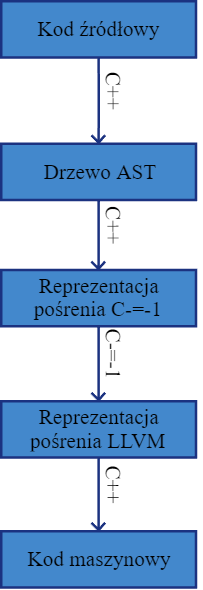
\includegraphics[height=6cm]{../assets/toplevelcompilationprocess.png}
			 \end{center}
		\end{column}
	\end{columns}
\end{frame}

\begin{frame}
	\frametitle{Kompilacja przez interpretację}

	\begin{figure}
		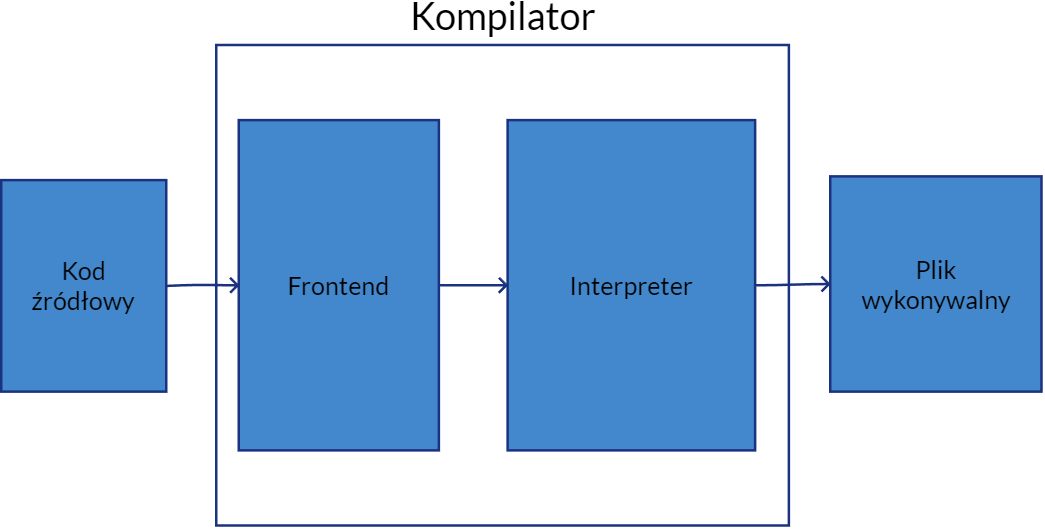
\includegraphics[width=\textwidth]{../assets/compilerouterdiagram.png}
	\end{figure}

\end{frame}

\begin{frame}
	\frametitle{Kompilacja przez interpretację}

	\begin{itemize}
		\item Budowana jest reprezentacja pośrednia programu.
		\item Komponent kompilujący do kodu maszynowego jest napisany w języku docelowym i jest interpretowany.
		\item Interpreter udostępnia narzędzia do budowy kodu maszynowego
		\item Komponent kompilujący może być wymieniany przez użytkownika
	\end{itemize}

\end{frame}


\section{Wyniki}

\begin{frame}
	\frametitle{Prędkość}

	\begin{itemize}
		\item Zaimplementowany kompilator jest bardzo wolny
		\item 10 minut, aby skompilować ~200 linii kodu\begin{itemize}
			\item Duża część kodu kompilatora jest interpretowana
			\item Interpreter używa nieefektywnych struktur danych
			\item Implementacja interpretera jest bardzo prosta
			\item Używany parser jest generyczny
		\end{itemize}
	\end{itemize}

\end{frame}

\begin{frame}[fragile]
	\frametitle{Wykonywanie metaprogramowania}

	\begin{lstlisting}
fn print<T>(object: T*) {
	if(isPrimitive(typeof(T)))
		printPrimitive(object);
	else
	{
		for(field : typeof(T).fields)
		{
			printPrimitive(field.name);
			printPrimitive(" value is: ");
			print<field.type>(field.getValue(object));
		}
	}
}
	\end{lstlisting}

\end{frame}

\begin{frame}
	\frametitle{Wykonywanie metaprogramowania}

\begin{itemize}
	\item Wywołanie metafunkcji wygląda tak jak zwykłej procedury
	\item Wywoływanie niektórych funkcji nie ma sensu w trakcie kompilacji, nawet jeśli jest to możliwe\begin{itemize}
		\item Manipulacja plikami
		\item Interakcja z użytkownikiem
	\end{itemize}
	\item Śledzenie czy zmienna pozostaje stała jest trudne
\end{itemize}

\end{frame}

\begin{frame}
	\frametitle{Wnioski: nowe możliwości}

	\begin{itemize}
		\item W pracy zaprezentowano kilka praktycznych aplikacji proponowanych mechanizmów\begin{itemize}
			\item Generowanie plików nagłówkowych dla języka C
			\item Adnotacja no discard
			\item Automatyczna generacja typów wyliczeniowych typu flagi (w czasie realizacji)
		\end{itemize}
		\item C-=-1 dużo łatwiej rozszerzyć niż inne, podobne języki
		\item Biblioteki w C-=-1 łatwiej użyć z innego języka niż na przykład C++
	\end{itemize}

\end{frame}

\begin{frame}
	\frametitle{Wnioski: system typów}

	\begin{itemize}
		\item System typów jest wzorowany na C++/C\#\begin{itemize}
			\item Generyki/szablony dodane po fakcie
			\item Nie korzysta z pełnych możliwości współczesnej teorii
		\end{itemize}
		\item Adnotacje powinny być częścią systemu typów\begin{itemize}
			\item Implementacja atrybutu const i pochodnych
		\end{itemize}
		\item Relacja pomiędzy adnotacjami a generykami wymaga więcej pracy
	\end{itemize}

\end{frame}

\begin{frame}[fragile]
	\frametitle{Wnioski: system typów}

	\begin{columns}
		\begin{column}{0.5\textwidth}
			\begin{lstlisting}[caption={const w C-=-1}]
fn main() -> usize
{
 [const()] let x = 3;
 let list = List<usize*>();
 list.push(&x);
 [const()] let pointer = &x;
}
			\end{lstlisting}
		\end{column}
		\begin{column}{0.5\textwidth}
			\begin{lstlisting}[caption={const w C++}]
int main()
{
 auto x = 3;
 auto list = std::vector<int const*>();
 list.push_back(&x);
 auto const* pointer = &x;
}

			\end{lstlisting}
		\end{column}
	\end{columns}
\end{frame}



\begin{frame}
	\frametitle{Wnioski}

	\begin{itemize}
		\item Celem pracy było zbadanie jak zaproponowane mechanizmy wpływają na programowanie\begin{itemize}%todo: wording
			\item Z braku czasu, zaimplementowano minimalny podzbiór języka
			\item Badania zaproponowanego języka są raczej powierzchowne
		\end{itemize}
		\item To co zostało przetestowane, wskazuje nowe kierunki badań\begin{itemize}
			\item Jaka powinna być relacja między atrybutami a systemem typów?
			\item Czy kompilator może działać z akceptowalną prędkością?
		\end{itemize}
		\item Pozostają dalsze badania nad wpływem tej formy metaprogramowania na tworzenia aplikacji.
	\end{itemize}

\end{frame}



\end{document}
	